\pagestyle{Uni}

\chapter{Requirements specification}

\section{User Stories}
\textbf{Menu:}
	\begin{itemize}
		\item As a User, I can create a game
		\begin{itemize}
			\item As a User, I can change the size of the board when creating a game
			\item As a User, I can change the map type of the board when creating a game
		\end{itemize}
		\item As a User, I can join a game
		\item As a User, I can spectate a game
		\item As a User, I can change my personal settings
		\begin{itemize}
			\item As a User, I can change my name
			\item As a User, I can change my avatar
		\end{itemize}
		\item As a User, I can read the rules
		\begin{itemize}
			\item As a User, I can search the rules
		\end{itemize}
	\end{itemize}

	\textbf{In-game:}
	\begin{itemize}	
		
		\item As a User, I can take an action
		\begin{itemize}
			\item As a User, I can move a space
			\item As a User, I can attack a monster
		\end{itemize}
		
		\item As a User, I can see stats
		\begin{itemize}
			\item As a User, I can see my stats
			\item As a User, I can see other players stats
			\item As a User, I can see monster stats
		\end{itemize}
		\item As a User, I have vision
		\begin{itemize}
			\item As a User, I can see the tiles in range around me and other players and if there is a item/monster placed on them.
			\item As a User, I can see the what kind of tile a tile holds if I or another player have passed it earlier on but no longer is in range of it.
			\item As a User, I can't see tiles that I or another player have not yet been in range of.
		\end{itemize}
	\end{itemize}

\section{Non-functional requirements}


\section{Vision}
	The vision with the project is to make a social game that is played as co-op so that a fellow-felling is created.  The game is intended for physical attendance where each player has their own android device. However, it is also possible to play online with friends, since all communication is intended to be happening over the Internet. In the following sections there are various Personans and scenarios that will try to give an impression on how a product like the one to be developed could be used.


\section{Personas}
\textbf{Christian} is 25 years old and lives in the hearth of Aarhus, he is dreaming of becoming a teacher. He loves to sit together with his friends late into the evening and play board games at a friends place, as the location is better and there is more room. Christian is quite technology interested and he always has the latest Samsung phone. In addition, he loves to spend his spare time playing computer games. The way he gets around in Aarhus is by using his bike. Christian owns the game that the group of friends all think is the most fun to play but he is tired of having to transport the game back and forth as it rather unhandy.

\textbf{Lærke} is 23 years old and lives in Manchester, she is currently an exchange students during her education in state economics. Lærke is very socially established and has a lot of good friends in Denmark. She keeps in touch with her friends in Denmark by using her android tablet to play different games.

\section{Scenarios}
\textbf{Christian}:
It is Thursday evening and Christian has taken his board game under his arm, like he does every Thursday and mounted his bike. Before he hits Thomas's house, he bikes towards Netto to get ready for a long evening. However, he thinks it's annoying to drag the game through Netto and in addition, it also limits the amount of supplies he can carry on his bike. When Christian arrives at Thomas and opens the game box, he can see how all the cards are messed up after the bike ride, after a while they have finally got all the content of the box sorted and can start playing. After playing for a while, a friend makes an unauthorized move, which is first discovered later. This move annoys Christian, as this will have an impact on the outcome of the game. Late in the evening they will have to stop the game as they go to school the next day and have to write down how far they have come.

\textbf{Lærke}:
It is Friday evening and Lærke can not afford to go out to town. Instead, she opens her tablet and finds the "Play store" to find a new co-op game she can play with her Danish friends. She finds the game "BackFight". Lærke writes to her Danish friends if they want to play with her. They quickly download the game and start a game. Time flies away and they are doing their second game, unfortunately, they have to stop when one of them need to wake up early the next day. The following day, they all want to continue the game. They open the app and choose their game from the day before and can continue from where they stopped.

\section{User interface design}
This section will show the ideas about how the application was supposed to look and feel when the design was made in the very start of the project.

On \ref{navigation} we see the flow from the main menu and how to create a game and start it.

\begin{figure}
	\centering
	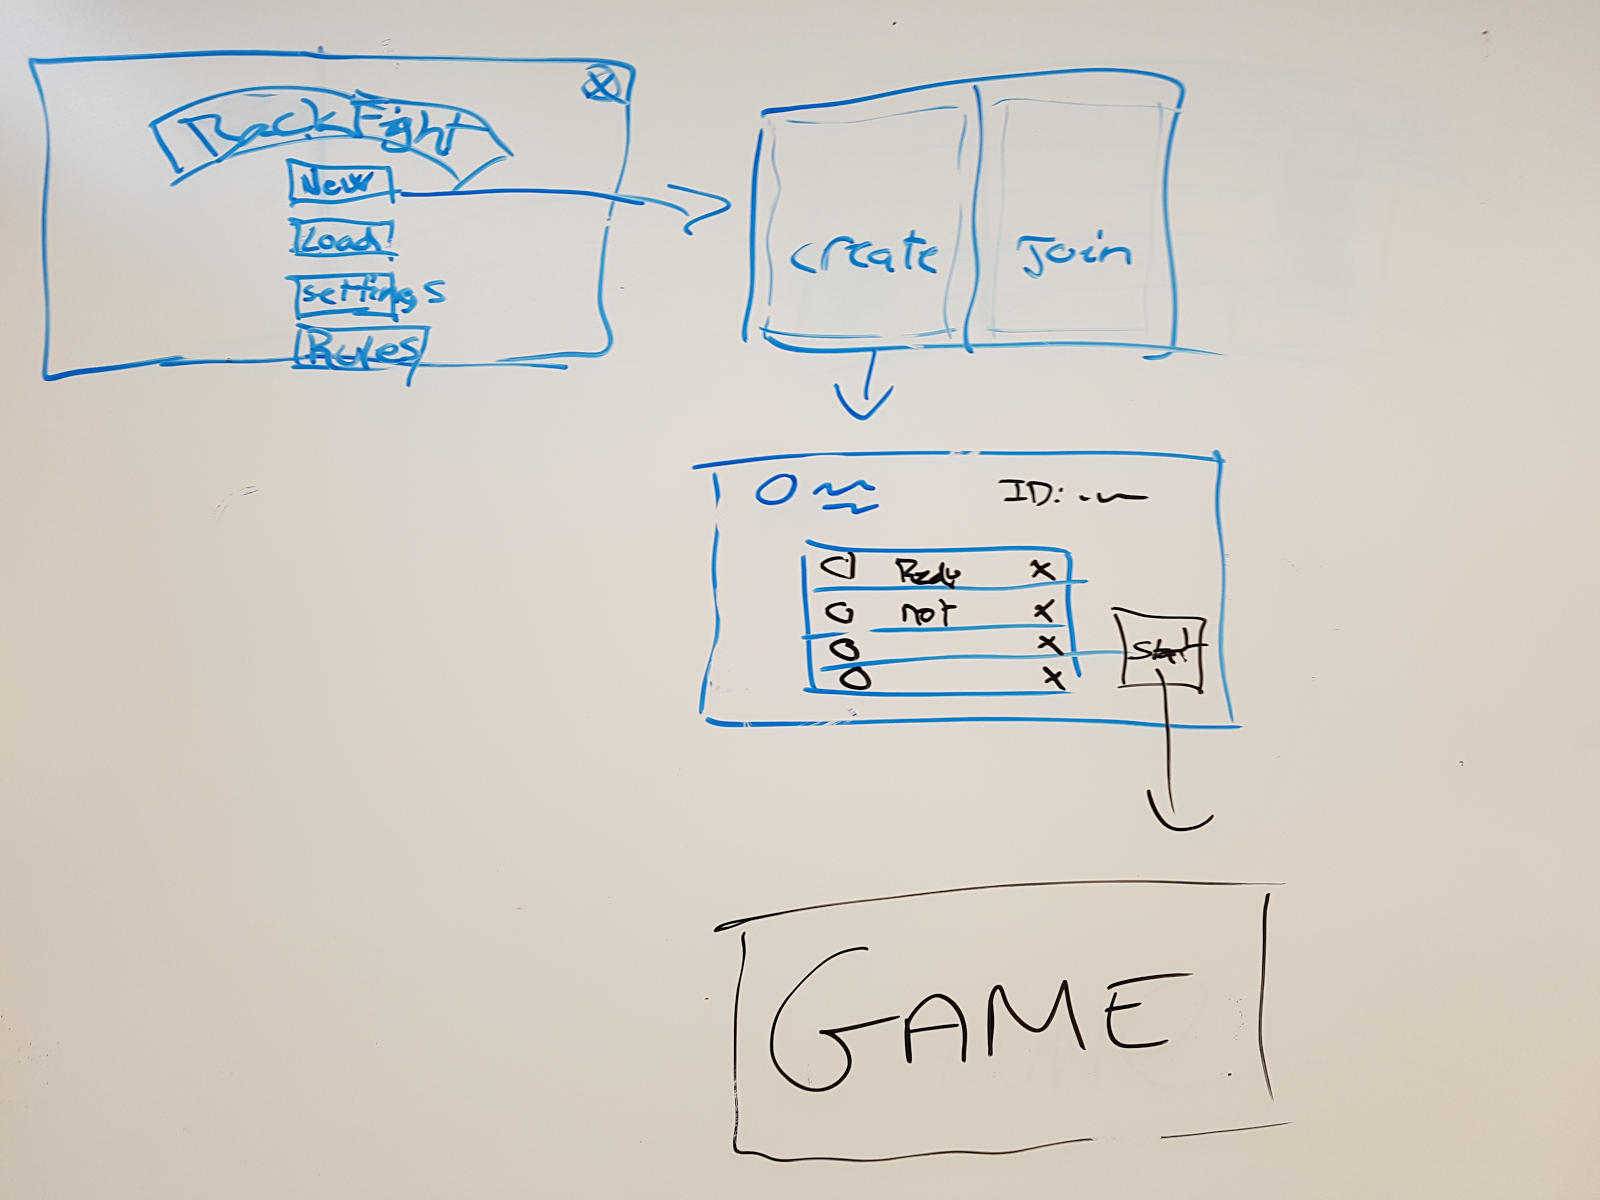
\includegraphics[width=130mm]{images/Gui.png}
	\caption{Menu navigation \label{navigation}}
\end{figure}


On \ref{gameLayout} the game view is seen as it was original planed it has been changed a bit under development but the idea of using tiles and players is still the same. There has been added some text to describe rounds and actions left.

\begin{figure}
	\centering
	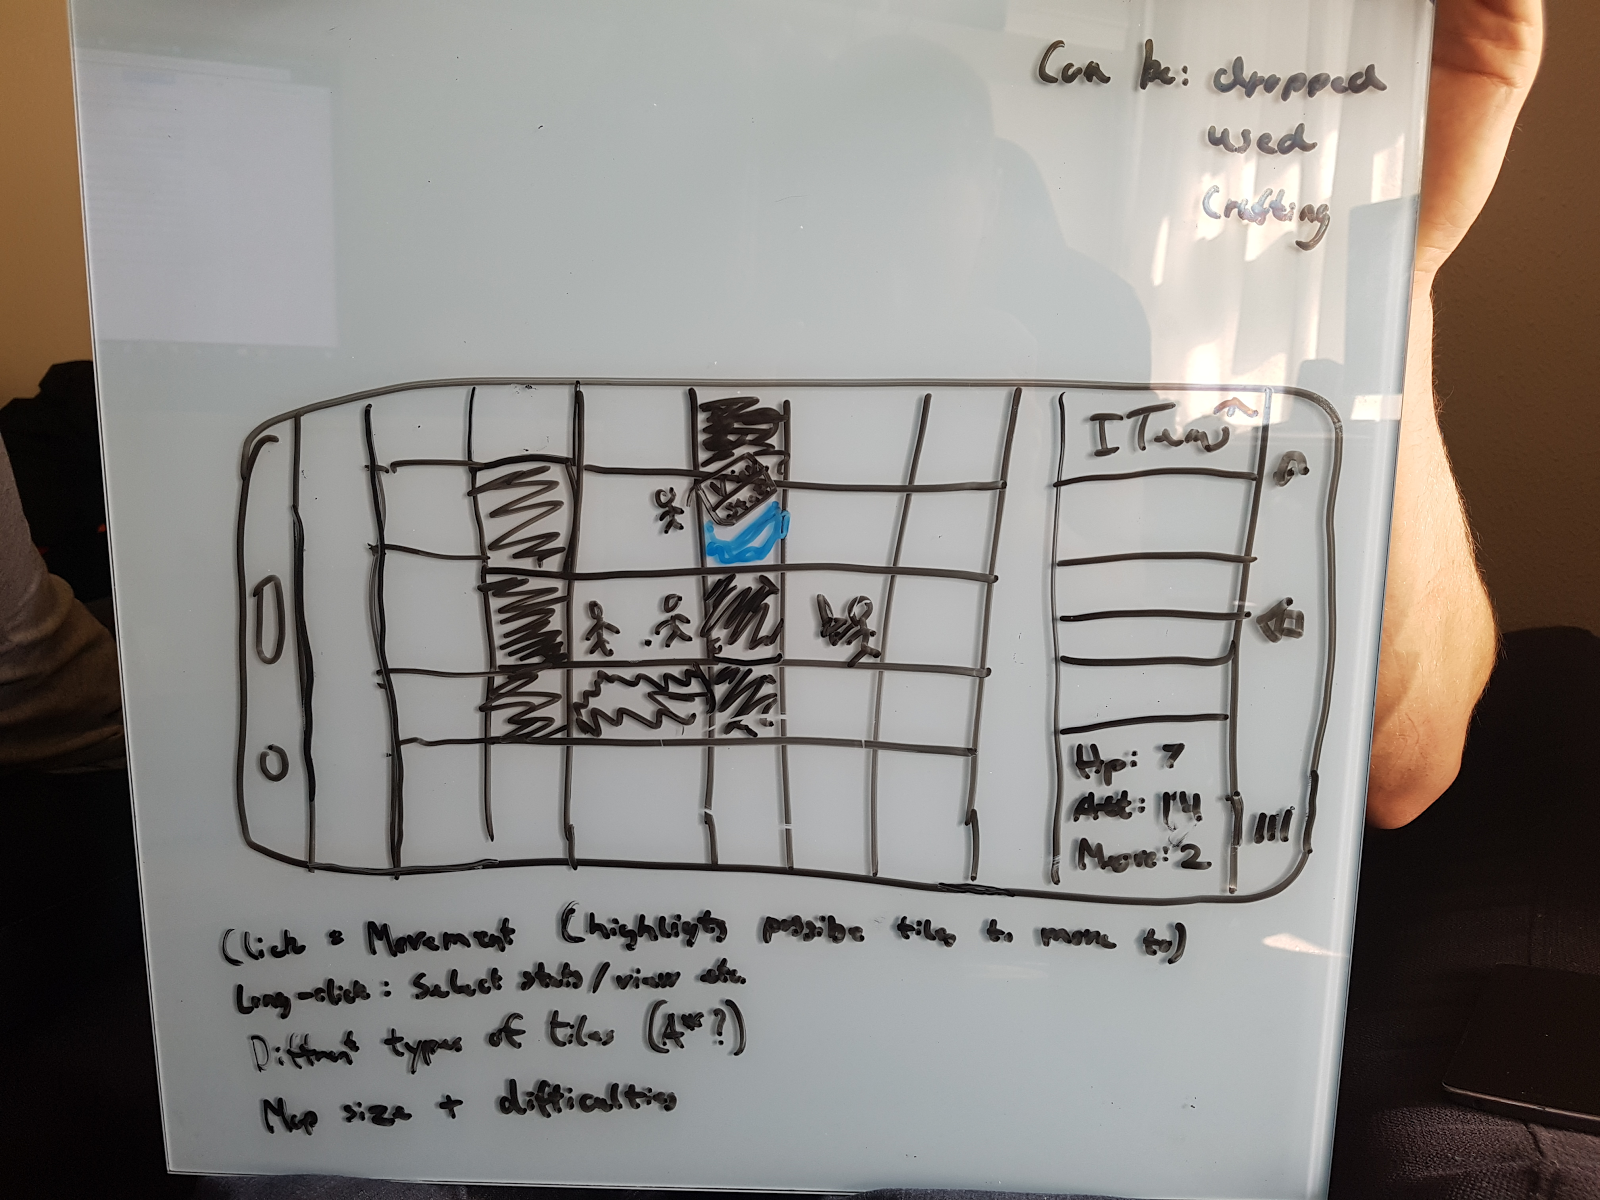
\includegraphics[width=130mm]{images/GameView.png}
	\caption{Game layout \label{gameLayout}}
\end{figure}

